\documentclass{beamer}\usepackage{graphicx, color}
%% maxwidth is the original width if it is less than linewidth
%% otherwise use linewidth (to make sure the graphics do not exceed the margin)
\makeatletter
\def\maxwidth{ %
  \ifdim\Gin@nat@width>\linewidth
    \linewidth
  \else
    \Gin@nat@width
  \fi
}
\makeatother

\IfFileExists{upquote.sty}{\usepackage{upquote}}{}
\definecolor{fgcolor}{rgb}{0.2, 0.2, 0.2}
\newcommand{\hlnumber}[1]{\textcolor[rgb]{0,0,0}{#1}}%
\newcommand{\hlfunctioncall}[1]{\textcolor[rgb]{0.501960784313725,0,0.329411764705882}{\textbf{#1}}}%
\newcommand{\hlstring}[1]{\textcolor[rgb]{0.6,0.6,1}{#1}}%
\newcommand{\hlkeyword}[1]{\textcolor[rgb]{0,0,0}{\textbf{#1}}}%
\newcommand{\hlargument}[1]{\textcolor[rgb]{0.690196078431373,0.250980392156863,0.0196078431372549}{#1}}%
\newcommand{\hlcomment}[1]{\textcolor[rgb]{0.180392156862745,0.6,0.341176470588235}{#1}}%
\newcommand{\hlroxygencomment}[1]{\textcolor[rgb]{0.43921568627451,0.47843137254902,0.701960784313725}{#1}}%
\newcommand{\hlformalargs}[1]{\textcolor[rgb]{0.690196078431373,0.250980392156863,0.0196078431372549}{#1}}%
\newcommand{\hleqformalargs}[1]{\textcolor[rgb]{0.690196078431373,0.250980392156863,0.0196078431372549}{#1}}%
\newcommand{\hlassignement}[1]{\textcolor[rgb]{0,0,0}{\textbf{#1}}}%
\newcommand{\hlpackage}[1]{\textcolor[rgb]{0.588235294117647,0.709803921568627,0.145098039215686}{#1}}%
\newcommand{\hlslot}[1]{\textit{#1}}%
\newcommand{\hlsymbol}[1]{\textcolor[rgb]{0,0,0}{#1}}%
\newcommand{\hlprompt}[1]{\textcolor[rgb]{0.2,0.2,0.2}{#1}}%

\usepackage{framed}
\makeatletter
\newenvironment{kframe}{%
 \def\at@end@of@kframe{}%
 \ifinner\ifhmode%
  \def\at@end@of@kframe{\end{minipage}}%
  \begin{minipage}{\columnwidth}%
 \fi\fi%
 \def\FrameCommand##1{\hskip\@totalleftmargin \hskip-\fboxsep
 \colorbox{shadecolor}{##1}\hskip-\fboxsep
     % There is no \\@totalrightmargin, so:
     \hskip-\linewidth \hskip-\@totalleftmargin \hskip\columnwidth}%
 \MakeFramed {\advance\hsize-\width
   \@totalleftmargin\z@ \linewidth\hsize
   \@setminipage}}%
 {\par\unskip\endMakeFramed%
 \at@end@of@kframe}
\makeatother

\definecolor{shadecolor}{rgb}{.97, .97, .97}
\definecolor{messagecolor}{rgb}{0, 0, 0}
\definecolor{warningcolor}{rgb}{1, 0, 1}
\definecolor{errorcolor}{rgb}{1, 0, 0}
\newenvironment{knitrout}{}{} % an empty environment to be redefined in TeX

\usepackage{alltt}
\usetheme{Stats}
\setbeamercovered{transparent}
\usepackage{color}
\usepackage{hyperref}
  \hypersetup{
  	colorlinks=true
		linkcolor=black
		}
\usepackage{url}
\usepackage{graphics}
\usepackage{tikz}
\usepackage{booktabs}





%%%%%%%%%%%%%%%%%%%%%%%%%%%%%%%% Title Slide %%%%%%%%%%%%%%%%%%%%%%%%%%
\title[]{Intro to Social Science Data Analysis \\[1cm] Research Question Design \& Data Download}
\author[]{
    \href{mailto:gandrud@yonsei.ac.kr}{Christopher Gandrud}
}
\date{\today}


\begin{document}

\frame{\titlepage}

\section[Outline]{}
\frame{\tableofcontents}

%%%%%%% Recap
\frame{
  \frametitle{Quick Quiz 1}
  What are the \textbf{three} minimum criterion for establishing a \textbf{causal relationship}?
}

\frame{
  \frametitle{Quick Quiz 2}
  Why do we often need to use tools for \textbf{statistical control}?\\[0.5cm]
  What is the main tool we learned last week for statistical control?
}

\frame{
  \frametitle{Quick Quiz 3}
  What is a reference category?
}

\frame{
  \frametitle{Quick Quiz 4}
  Why do King et al. (2000) recommend simulating expected outcomes and graphing the results?
}

\begin{frame}[fragile]
  \frametitle{Simulating Expected Values for Categorical Variables}
\begin{knitrout}
\definecolor{shadecolor}{rgb}{0.969, 0.969, 0.969}\color{fgcolor}\begin{kframe}
\begin{alltt}
\hlfunctioncall{library}(openintro)
\hlfunctioncall{library}(Zelig)

\hlfunctioncall{data}(hsb2)

M1 <- \hlfunctioncall{zelig}(read ~ \hlfunctioncall{as.factor}(gender) 
            + write, model = \hlstring{"normal"}, 
            data = hsb2, cite = FALSE)

Values <- \hlfunctioncall{c}(\hlstring{"male"}, \hlstring{"female"})

XOut <- \hlfunctioncall{setx}(M1, gender = Values)

ZSim <- \hlfunctioncall{sim}(M1, XOut)
\end{alltt}
\end{kframe}
\end{knitrout}

\end{frame}

\begin{frame}[fragile]
  \frametitle{Plot Expected Values}
\begin{knitrout}
\definecolor{shadecolor}{rgb}{0.969, 0.969, 0.969}\color{fgcolor}\begin{kframe}
\begin{alltt}
\hlfunctioncall{plot}(ZSim)
\end{alltt}
\end{kframe}

{\centering 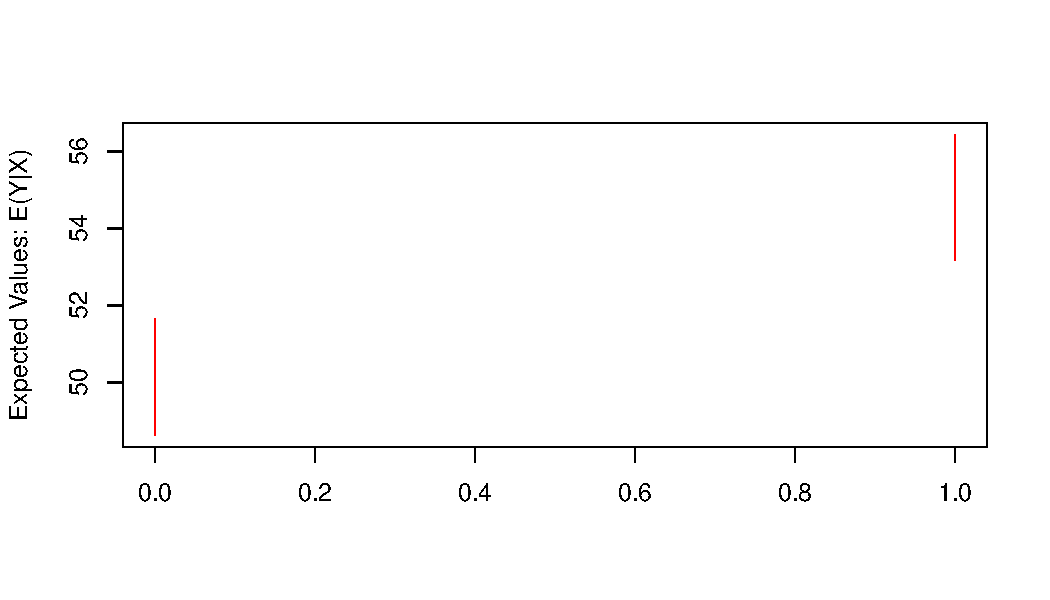
\includegraphics[width=\maxwidth]{figure/PlotExpected} 

}


\end{knitrout}

\end{frame}



%%%%%%%%% Research Project: Goals
\section{Research Project: Goals}
\frame{
  \frametitle{Pair Research Project: Goals}
{\LARGE{\textbf{Goals:}}} \\[0.5cm]
  With a partner, answer a \textbf{social science research question} primarily using the \textbf{data analysis tools} covered in this course. \\[0.5cm]
  Present your results in both a:
  \begin{itemize}
    \item<1-> \textbf{short paper} (max 1,000 words),
    \item<1-> \textbf{short presentation} (max 15 minutes).
  \end{itemize} \\[0.5cm]
  As always, it must be \textbf{reproducible}.
}

\frame{
  \frametitle{Schedule}
  We are dedicating \textbf{all} of the class time for the rest of the course to the research project. \\[0.5cm]
  Schedule:
  \begin{itemize}
    \item<2-> Week 13: Research question, design, \& data download,
    \item<3-> Week 14: Statistical Analysis \& Results Visualization,
    \item<4-> Week 15: Write up.
    \item<5-> Week 16: Presentations.
  \end{itemize}
}

\frame{
	\frametitle{Pair Research Project}
  {\LARGE{\textbf{Due:}}} \\[0.5cm]
  \begin{itemize}
    \item Paper: 18 December
    \item Presentation: 19 or 21 December
  \end{itemize}
}

%%%%%%%%%% Paper Structure
\section{Paper Structure}
\frame{
  \frametitle{Paper Structure}
  Your paper should have the following structure: \\[0.5cm]
  \begin{itemize}
    \item \textbf{Introduction}: Research Question, Thesis Statement, Paper Outline.
    \item \textbf{Literature Review}: Brief discussion of previous research on this topic (including possible alternative explanations).
    \item \textbf{Data \& Methods}: Describe the data you collected (sources, variable meaning) \& the methods that you use to test your hypothesis.
    \item \textbf{Results}: Show and discuss you results.
    \item \textbf{Conclusion:} Wrap up \& discuss your research \textbf{limitations}.
  \end{itemize}
}

\frame{
  \frametitle{Presentation Structure}
{\LARGE{Note:}} \\[0.5cm]
  Your presentation's structure will mostly be the same as your paper's.
}

%%%%%%%%%%%%% Research Question \& Research Design
\section{Research Question \& Research Design}
\frame{
  \frametitle{Research Question \& Research Design}
{\LARGE{This week:}} \\[0.5cm]
  You will develop your research question and the research design you will use to try to answer it. \\[0.5cm]
  This is \textbf{Assignment 4}.
}

\begin

\section{Assignment 4}
\frame{
  \frametitle{Assignment 4}
  Due: Friday 30 November \\[0.5cm]
  {\Large{Research Design}} \\[0.25cm]
  With your partner plan your research by answering the following questions:
  \begin{enumerate}
    \item What \textbf{difference} do you want to explain?
    \item What is your \textbf{best guess} explanation (i.e. thesis statement)?
    \item Can you \textbf{test your hypothesis using data}? If so, what data do you need to collect and what tests could you use?
    \item What \textbf{rival explanations} are their?
    \item How could you use data to test whether your best guess or the rival explanations are better? Write this as an \textbf{equation}.
  \end{enumerate}
{\tiny{Questionnaire from: modified from Cheryl Schonhardt-Bailey}}
}

\end{document}
